\chapter{Symmetrien der Geradenkonfiguration} \label{chap:configsymm}
Die hohe Zahl an Geraden auf \textsc{Fermat}-Flächen legt es nahe, dass ihre Struktur durch die Geraden in hohem Maß festgelegt wird. Hier wollen wir den Zusammenhang untersuchen zwischen semilinearen Symmetrien der Fläche und Permutationen der Geraden, die das Schnittverhalten respektieren.

Wir führen für dieses Kapitel neue Notation ein: den Primkörper von $K$ bezeichnen wir als $k$. Ohne Einschränkung sei $K = \overline k$ angenommen: offenbar sind alle Geraden über $\overline k$ definiert.

\section{Lineare und Kombinatorische Symmetrien}
Die Fermat-Flächen haben einen hohen Grad an Symmetrie. Offenbar lassen sowohl Permutationen der Koordinaten als auch Multiplikation der Koordinaten mit $d$-ten Einheitswurzeln die Fläche invariant. Das sind alles lineare Transformationen, diese reichen aber nicht, um alle Symmetrien der Geradenkonfiguration zu erklären. Dazu müssen wir noch die Automorphismengruppe von $K$ hinzunehmen. Also operieren die Gruppen $S_4$, $\Gal K/k$ und $\mu_d^4$, in letzterer operiert eine Untergruppe isomorph zu $\mu_d$ trivial: Multiplikation aller Koordinaten mit derselben Einheitswurzel ändert nichts. Die Gruppen schneiden sich nur in $\{\id\}$, also haben wir eine Aktion von
\begin{equation}
\mu_d^4 / \mu_d \rtimes (S_4 \times \Gal K/k) \subset \PGaL 4K,
\end{equation}
auf $F_d$, wobei der Homomorphismus $S_4 \times \Gal K/k \rightarrow \Aut(\mu_d^4 / \mu_d)$ so definiert ist: $(\sigma, \tau)$ wird abgebildet auf $\mu_d^4 / \mu_d \to \mu_d^4 / \mu_d$, $(x_0:\dots:x_3) \mapsto (\tau(x_{\sigma(0)}):\dots:\tau(x_{\sigma(3)}))$. Wenn es Geistergeraden gibt, treten sogar noch mehr Symmetrien auf, wie wir später sehen werden.

\begin{defin}
Sei $S \in \proj n(K)$ eine beliebige Menge. Als semilineare Symmetriegruppe von $S$ bezeichnen wir die Untergruppe
\begin{equation}
G_l = G_l(S) = \{ g \in \PGaL{n+1}K: gS = S \} \subset \PGaL{n+1}K.
\end{equation}
\end{defin}

Solche semilinearen Abbildungen lassen nicht nur die Fläche invariant, sondern schicken auch Geraden auf Geraden. Damit permutieren sie die Geraden auf der Fläche, offenbar bleibt dabei aber ihre Schnittkonfiguration erhalten. Die Schnittkonfiguration wird durch einen Graphen $\mathcal G = (L,E)$ kodiert, dabei ist die $L$ die Menge der Geraden, und $(l_1, l_2) \in E$, wenn $l_1$ und $l_2$ sich schneiden.

Die Frage liegt nahe, welche Permutationen der Geraden es denn gibt, die die Schnittkonfiguration erhalten.
\begin{defin}
Sei nun $S \in \proj 3(K)$ eine projektive Fläche, $\mathcal G = (L,E)$ die Geradenkonfiguration. Dann ist die kombinatorische Symmetriegruppe von $S$ die Automorphismengruppe des Graphen $\mathcal G$, d.h.
\begin{equation}
G_k = G_k(S) = \{ \sigma \in \Sym(L): (l_1, l_2) \in E \Leftrightarrow (\sigma(l_1), \sigma(l_2)) \in E \}
\end{equation}
\end{defin}

Wir wollen in diesem Kapitel die Beziehung zwischen diesen beiden Gruppen ausarbeiten. Wie oben bemerkt, induziert jede lineare Symmetrie eine kombinatorische, also haben wir einen Homomorphismus $G_l(F_d) \to G_k(F_d)$. Wir berechnen zunächst den Kern, und zeigen später Surjektivität. Die folgende Betrachtung ist inspiriert durch \cite[Bem.~4.10.1, S.~404]{Hartshorne}, und \cite[Aufg. C--D, S.~180]{Mumford}. Dort wird die Situation für allgemeine reguläre Flächen dritten Grades untersucht.

An dieser Stelle bemerken wir, dass $\GaL 4K = \GL 4K \rtimes \Aut K$ und $\PGaL 4K = \PGL 4K \rtimes \Aut K$.\footnote{Das folgt leicht aus den Bemerkungen in \cite[S.~2--3]{Dieudonne}.}

\begin{lemma}
Gibt es unter den Schnittpunkten der Geraden auf $S$ mindestens fünf in allgemeiner Lage,\footnote{das heißt: keine vier davon liegen auf einer projektiven Ebene.} so besteht der Kern des Homomorphismus $G_l(S) \to G_k(S)$ in einer geeigneten Basis nur aus Automorphismen von $K$.
\end{lemma}
\begin{proof}
Sei $g \in \PGaL 4K$ so gewählt, dass alle Geraden auf $S$ auf sich selbst abgebildet werden. Dann werden auch die fünf Schnittpunkte auf sich selbst abgebildet. Sei $(A, \sigma) \in \GaL 4K = \GL 4K \rtimes \Aut K$ ein Urbild von $g$ und $v_1, \dots, v_5$ Urbilder der Schnittpunke in $K^4$, dann gilt also $(A, \sigma)v_i = \lambda_i v_i$ mit $\lambda_i \in K^*$. Sei $P$ die Matrix mit den Spalten $v_1, \dots, v_4$, dann bildet also $(P^{-1},\id)(A,\sigma)(P,\id) = (P^{-\sigma}AP,\sigma)$ die Basisvektoren auf Vielfache ihrer selbst ab. Folglich hat die Matrix $P^{-\sigma}AP$ Diagonalgestalt. (Hier ist $P^{-\sigma}$ eine Kurzschreibweise für $(P^{-1})^\sigma$.)

Betrachte nun den Vektor $v_5 \in K^4 \setminus 0$ zum fünften Schnittpunkt. In der Basis $\{v_i\}_{i<5}$ hat $v_5$ dann die Gestalt $\sum_i \alpha_i v_i$ mit $\alpha_i \neq 0$ für alle $i$, da die fünf Schnittpunkte in allgemeiner Lage sind. Nun gilt aber $(A,\sigma) v_5 = \lambda_5 v_5$, oder $(P^{-\sigma}AP,\sigma)(\alpha_1,\dots,\alpha_4) = \lambda_5(\lambda_1\alpha_1,\dots,\lambda_4\alpha_4)$. Damit sind die Diagonaleinträge $\lambda_1, \dots, \lambda_4$ der Matrix $P^{-\sigma}AP$ alle gleich $\lambda$, da die $\alpha_i$ nicht verschwinden. Also ist $P^{-\sigma}AP = \lambda \id$, mithin ist $g$ zu $(\id, \sigma)$ linear konjugiert. Man beachte dabei, dass $P$ unabhängig von $g$ ist: man kann also durch einen Basiswechsel alle Elemente des Kerns gleichzeitig auf die Form $(\id, *)$ bringen.
\end{proof}
Wie wir weiter unten sehen werden, schneiden sich zwei Geraden einer Klasse in Punkten der Form $(1:\zeta^n:0:0)$, $\zeta \in \mu_{2d}$ primitiv und $n$ ungerade; sowie Permutationen der Koordinaten. Durch Probieren findet man damit leicht fünf Punkte in allgemeiner Lage. Die fünf $4 \times 4$-Untermatrizen von
\begin{equation*}
\begin{pmatrix}
1 & 0 & 1 & 0 & 1 \\
\zeta & 0 & 0 & 1 & 0 \\
0 & 1 & \zeta^3 & 0 & 0 \\
0 & \zeta & 0 & \zeta^5 & \zeta^3 \\
\end{pmatrix}
\end{equation*}
haben Determinanten $(\zeta^2-1)\zeta^4$, $(\zeta+1)\zeta^4$, $-(\zeta^3+1)\zeta^3$, $-(\zeta^3+1)\zeta^6$ bzw.~$(\zeta+1)\zeta^3$. Für $d>3$ verschwindet keine davon. Im Folgenden nehmen wir die ersten drei Vektoren als Basis.

Nun müssen wir noch ermitteln, welche Automorphismen im Kern liegen. Offenbar gilt im Fall der regulären Geraden $\Gal K/{k(\mu_{2d})} \subset \ker(G_l \to G_k)$, gibt es Geistergeraden, dann $\Gal K/{k(\mu_{d(d-2)})} \subset \ker(G_l \to G_k)$. Wir wollen nun zeigen, dass der Kern nicht größer ist.
\begin{lemma}
Sei $E$ die Körpererweiterung von $k$, die durch die Quotienten der \textsc{Plücker}-Koordinaten der Geraden auf der Fläche $S$ erzeugt wird. Der Kern des Homomorphismus $G_l(S) \to G_k(S)$ ist dann $\Gal K/E$.
\end{lemma}
\begin{proof}
Sei die Basis des Raumes wie im vorigen Lemma gewählt, sodass $\ker(G_l \to G_k) \subset \Aut K$. Mit den Geraden sind auch die Schnittpunkte über $E$ definiert, die Verhältnisse der \textsc{Plücker}-Koordinaten der transformierten Geraden erzeugen daher auch $E$.

Da diese von einer semilinearen Symmetrie aus dem Kern fix gelassen werden sollen, müssen solche die Verhältnisse der \textsc{Plücker}-Koordinaten fix lassen. Damit folgt $\ker(G_l \to G_k) \subset \Gal K/E$. Die Umkehrung ist offensichtlich.
\end{proof}

Damit können wir den Kern explizit angeben: im Fall $d \neq p^n+1$, wenn also keine Geistergeraden existieren, ist $E = k(\mu_{2d})$. Weiter haben wir oben gesehen, dass $\mu_d^4 / \mu_d \rtimes (S_4 \times \Gal K/k) \subset G_l(F_d)$. Nun gilt nach elementarer \textsc{Galois}-Theorie
\begin{equation}
\Gal K/k \;/\; \Gal K/{k(\mu_{2d})} \cong \Gal k(\mu_{2d})/k;
\end{equation}
damit folgt, dass $G_k(F_d)$ eine Untergruppe isomorph zu $\mu_d^4 / \mu_d \rtimes (S_4 \times \Gal \mathbb Q(\mu_{2d})/{\mathbb Q})$ enthält. Wir wollen im nächsten Abschnitt zeigen, dass sogar Gleichheit gilt.

\section{Reguläre Geraden}
\paragraph{Konfiguration} Wir schreiben die Geraden aus \eqref{eq:regular} mit einer fixierten primitiven Einheitswurzel $\zeta \in \mu_{2d}$ und $a,b \in (2\mathbb Z + 1)/2d\mathbb Z \subset \Zmod 2dZ$:
\begin{equation}
\begin{split}
\Lcl(I)_{a,b}  :\qquad	&\langle (1,\zeta^a,0,0), (0,0,1,\zeta^b)\rangle \\
\Lcl(II)_{a,b} :\qquad	&\langle (1,0,\zeta^a,0), (0,1,0,\zeta^b)\rangle \\
\Lcl(III)_{a,b}:\qquad	&\langle (1,0,0,\zeta^a), (0,1,\zeta^b,0)\rangle.
\end{split}
\end{equation}
Ob sich zwei verschiedene projektive Geraden schneiden, stellt man anhand der Determinante der Matrix aus ihren vier Basisvektoren fest: verschwindet sie, dann hat die Matrix nicht vollen Rang, also schneiden sie sich in einem projektiven Punkt.

Damit überlegt man sich leicht, dass sich zwei Geraden aus derselben Familie genau dann schneiden, wenn sie in einem der beiden Parameter $a$, $b$ übereinstimmen. Für Geraden aus verschiedenen Klassen ergibt sich folgendes: zwei Geraden $\Lcl(I)_{a,b}$ und $\Lcl(II)_{a',b'}$ schneiden sich, wenn
\begin{equation}
\det \begin{pmatrix}
1 & \zeta^a & 0 & 0 \\
0 & 0 & 1 & \zeta^b \\
1 & 0 & \zeta^{a'} & 0 \\
0 & 1 & 0 & \zeta^{b'}
\end{pmatrix} = 0 \quad\Longleftrightarrow\quad \zeta^{a'} \zeta^b = \zeta^a \zeta^{b'} \quad\Leftrightarrow\quad a-b \equiv a'-b' \pmod{2d}.
\end{equation}
Analog erhält man, dass sich $\Lcl(I)_{a,b}$ und $\Lcl(III)_{a'',b''}$ schneiden, wenn $a''-b'' \equiv a+b$, und $\Lcl(II)_{a',b'}$ und $\Lcl(III)_{a'',b''}$, wenn $a''+b'' \equiv a'+b' \pmod{2d}$.

Wir wollen zur Beschreibung der Schnittkonfiguration noch einige Begriffe einführen: die drei Teilmengen von Geraden $\Lcl(I)$, $\Lcl(II)$ und $\Lcl(III)$ wollen wir Klassen nennen. Die Teilmengen davon mit konstantem Parameter $b$ nennen wir Zeilen, die mit konstantem Parameter $a$ Spalten. Dann bilden die Zeilen und Spalten vollständige Graphen $K_d$.

Teilmengen der Klassen mit konstanter Summe bzw. Differenz der Parameter $a$, $b$ mögen Diagonalen heißen. Bestimmte Diagonalen verschiedener Klassen bilden bipartite Graphen $K_{d,d}$. In der folgenden Grafik sind einige dieser Diagonalen dargestellt. Jede Gerade in einer der Diagonalen schneidet jede andere in der Diagonalen gleicher Farbe in der entsprechenden anderen Klasse.

\begin{figure}[h]
\centering
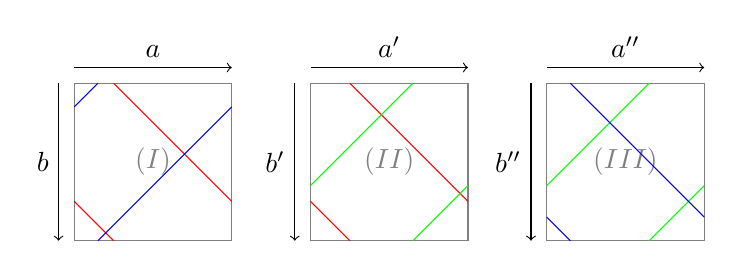
\begin{tikzpicture}
\draw[color=gray]
	[xshift=0cm] (0,0) rectangle (2,2) (1,1) node{$\Lcl(I)$}
	[xshift=3cm] (0,0) rectangle (2,2) (1,1) node{$\Lcl(II)$}
	[xshift=3cm] (0,0) rectangle (2,2) (1,1) node{$\Lcl(III)$};
\draw[->,xshift=0cm] (0,2.2) -- (2,2.2) node[above,midway] {$a$};
\draw[->,xshift=0cm] (-0.2,2) -- (-0.2,0)  node[left,midway] {$b$};
\draw[->,xshift=3cm] (0,2.2) -- (2,2.2) node[above,midway] {$a'$};
\draw[->,xshift=3cm] (-0.2,2) -- (-0.2,0)  node[left,midway] {$b'$};
\draw[->,xshift=6cm] (0,2.2) -- (2,2.2) node[above,midway] {$a''$};
\draw[->,xshift=6cm] (-0.2,2) -- (-0.2,0)  node[left,midway] {$b''$};
\draw[color=red]
	[xshift=0cm] (0.5,0) -- (0,0.5) (0.5,2) -- (2,0.5)
	[xshift=3cm] (0.5,0) -- (0,0.5) (0.5,2) -- (2,0.5);
\draw[color=green]
	[xshift=3cm] (1.3,0) -- (2,0.7) (0,0.7) -- (1.3,2)
	[xshift=3cm] (1.3,0) -- (2,0.7) (0,0.7) -- (1.3,2);
\draw[color=blue]
	[xshift=0cm] (0,1.7) -- (0.3,2) (0.3,0) -- (2,1.7)
	[xshift=6cm,yscale=-1,yshift=-2cm]
		(0,1.7) -- (0.3,2) (0.3,0) -- (2,1.7);
\end{tikzpicture}
\caption{Schnitte zwischen verschiedenen Klassen der regulären Geraden}\label{fig:reg}
\end{figure}

\paragraph{Symmetrien} Wir haben uns bereits klargemacht, dass wir auf $F_d$ eine Aktion der Gruppe $\mu_d^4 / \mu_d \rtimes (S_4 \times \Gal \mathbb Q(\mu_{2d})/{\mathbb Q})$ haben, die nach obiger Proposition auch auf der Geradenkonfiguration transitiv operiert. Machen wir uns zunächst klar, auf welche Weise das geschieht. Multiplikation der $i$-ten Koordinate mit $\zeta^{s_i}$, $s_i$ gerade, bewirkt offenbar eine Verschiebung der Konfiguration in den einzelnen Klassen, und zwar wie folgt:

\begin{figure}[h]
\centering
\begin{tikzpicture}
\draw[color=black]
	[xshift=0cm] (0,0) rectangle (2,2) (1,1) node{$\Lcl(I)$}
	[xshift=5cm] (0,0) rectangle (2,2) (1,1) node{$\Lcl(II)$}
	[xshift=5cm] (0,0) rectangle (2,2) (1,1) node{$\Lcl(III)$};
\draw[->,xshift=0cm] (0.5,2.2) -- (1.5,2.2) node[above,midway] {$+s_0$};
\draw[->,xshift=0cm] (-0.2,1.5) -- (-0.2,0.5) node[left,midway] {$+s_2$};
\draw[->,xshift=0cm] (1.5,-0.2) -- (0.5,-0.2) node[below,midway] {$+s_1$};
\draw[->,xshift=0cm] (2.2,0.5) -- (2.2,1.5) node[right,midway] {$+s_3$};

\draw[->,xshift=5cm] (0.5,2.2) -- (1.5,2.2) node[above,midway] {$+s_0$};
\draw[->,xshift=5cm] (-0.2,1.5) -- (-0.2,0.5) node[left,midway] {$+s_1$};
\draw[->,xshift=5cm] (1.5,-0.2) -- (0.5,-0.2) node[below,midway] {$+s_2$};
\draw[->,xshift=5cm] (2.2,0.5) -- (2.2,1.5) node[right,midway] {$+s_3$};

\draw[->,xshift=10cm] (0.5,2.2) -- (1.5,2.2) node[above,midway] {$+s_0$};
\draw[->,xshift=10cm] (-0.2,1.5) -- (-0.2,0.5) node[left,midway] {$+s_1$};
\draw[->,xshift=10cm] (1.5,-0.2) -- (0.5,-0.2) node[below,midway] {$+s_3$};
\draw[->,xshift=10cm] (2.2,0.5) -- (2.2,1.5) node[right,midway] {$+s_2$};
\end{tikzpicture}
\caption{Aktion von $\mu_d^4 / \mu_d$ auf der Geradenkonfiguration}\label{fig:coordmult}
\end{figure}

Die \textsc{Galois}-Automorphismen wirken ähnlich: der Automorphismus $\zeta \mapsto \zeta^t$ mit einer primitiven Einheitswurzel $\zeta \in \mu_{2d}$ und $t \in (\Zmod 2dZ)^*$ bewirkt eine Multiplikation der Indizes $a$, $b$ einer Klasse mit $t$.

\begin{figure}[h]
\centering
\begin{tikzpicture}
\draw[color=black]
	[xshift=0cm] (0,0) rectangle (2,2) (1,1) node{$\Lcl(I)$}
	[xshift=5cm] (0,0) rectangle (2,2) (1,1) node{$\Lcl(II)$}
	[xshift=5cm] (0,0) rectangle (2,2) (1,1) node{$\Lcl(III)$};
\draw[->>,xshift=0cm] (0.5,2.2) -- (1.5,2.2) node[above,midway] {$\phantom{x} \cdot t$};
\draw[->>,xshift=0cm] (-0.2,1.5) -- (-0.2,0.5) node[left,midway] {$\phantom{x} \cdot t$};

\draw[->>,xshift=5cm] (0.5,2.2) -- (1.5,2.2) node[above,midway] {$\phantom{x} \cdot t$};
\draw[->>,xshift=5cm] (-0.2,1.5) -- (-0.2,0.5) node[left,midway] {$\phantom{x} \cdot t$};

\draw[->>,xshift=10cm] (0.5,2.2) -- (1.5,2.2) node[above,midway] {$\phantom{x} \cdot t$};
\draw[->>,xshift=10cm] (-0.2,1.5) -- (-0.2,0.5) node[left,midway] {$\phantom{x} \cdot t$};
\end{tikzpicture}
\caption{Aktion von $\Gal \mathbb Q(\mu_{2d})/{\mathbb Q}$ auf der Geradenkonfiguration}\label{fig:galois}
\end{figure}

Die Aktion der Koordinatenpermutation ist schwieriger zu beschreiben. Man kann die drei Matrizen wie in Abb.~\ref{fig:perm} gezeigt auf einen Würfel kleben. Dann entspricht die Aktion der $S_4$ der Drehgruppe des Würfels.

\begin{figure}[h] % we might need transform canvas={...} or sloping and slanting node text (http://tex.stackexchange.com/questions/62038/text-placed-in-pespective-on-3d-object)
\centering
\begin{tikzpicture}[x  = {(0.9659cm,0.25882cm)},
                    y  = {(-0.5cm,0.5cm)},
                    z  = {(0cm,1cm)}, scale = 2]
\begin{scope}[canvas is yx plane at z=0]
  \path[draw=black] (0,0) rectangle (2,2);
  \path[fill=gray!80] (0.5,0.5) rectangle (1.5,1.5);
\end{scope}
\path (0,1,0) -- node[sloped, rotate=180, xslant=-0.6]{$\Lcl(III)$} (2,1,0);
\begin{scope}[canvas is zx plane at y=2]
  \path[draw=black] (0,0) rectangle (2,2);
  \path[fill=gray!80] (0.5,0.5) rectangle (1.5,1.5);
\end{scope}
\path (1,2,0) -- node[sloped, xslant=-0.4]{$\Lcl(I)$} (1,2,2);
\begin{scope}[canvas is zy plane at x=2]
  \path[draw=black] (0,0) rectangle (2,2);
  \path[fill=gray!80] (0.5,0.5) rectangle (1.5,1.5);
\end{scope}
\path (2,0,1) -- node[sloped, xscale=-1, xslant=0.8]{$\Lcl(II)$} (2,2,1);
\begin{scope}[canvas is zx plane at y=0]
  \path[draw=black] (0,0) rectangle (2,2);
  \path[fill=gray!50, fill opacity=0.5] (0.5,0.5) rectangle (1.5,1.5);
\end{scope}
\path (0,0,1) -- node[sloped, xslant=0.3]{$\Lcl(I)$} (2,0,1);
\begin{scope}[canvas is zy plane at x=0]
  \path[draw=black] (0,0) rectangle (2,2);
  \path[fill=gray!50, fill opacity=0.5] (0.5,0.5) rectangle (1.5,1.5);
\end{scope}
\path (0,1,2) -- node[sloped, yscale=-1, xslant=-0.8]{$\Lcl(II)$} (0,1,0);
\begin{scope}[canvas is yx plane at z=2]
  \path[draw=black] (0,0) rectangle (2,2);
  \path[fill=gray!50, fill opacity=0.5] (0.5,0.5) rectangle (1.5,1.5);
\end{scope}
\path (1,2,2) -- node[sloped, rotate=180, xslant=0.5]{$\Lcl(III)$} (1,0,2);
\end{tikzpicture}
\caption{Visualisierung der Aktion von $S_4$ auf der Geradenkonfiguration}\label{fig:perm}
\end{figure}

\paragraph{Vergleich der Symmetriegruppen} Wir zeigen nun, dass diese Symmetrien der Geradenkonfiguration die einzigen sind, die das Schnittverhalten respektieren. Zunächst müssen wir die Konfiguration aber genauer untersuchen.

\begin{lemma}
Sei $d \geq 4$, dann sind die einzigen Subgraphen isomorph zu $K_d$ die aus den Geraden einer Klasse bestehenden, die in einem der beiden Parameter übereinstimmen.
\end{lemma}
\begin{remarks}
Für $d=3$ ist das nicht der Fall: die drei Schnittpunkte der Diagonalen in Abb.~\ref{fig:reg} bilden ebenfalls einen $K_3$. (Die Grafik ist hier etwas irreführend: die Diagonalen schneiden sich für ungerades $d$ nur genau einmal.) \note Das ist etwas vage. Weglassen?
\end{remarks}
\begin{proof}
Sei $l \in L$ eine beliebige Gerade, dann schneidet sie jeweils $d-1$ Geraden in derselben Zeile bzw.~Spalte und jeweils $d$ Geraden in den entsprechenden Diagonalen in den anderen beiden Klassen. Wir wollen nun untersuchen, zu welchen vollständigen Graphen $K_d$ die Gerade $l$ gehört.

Von den $d$ Geraden in anderen Klassen, die $l$ schneiden, kann jeweils nur eine Teil des $K_d$ sein: denn diese schneiden sich untereinander nicht, da die Diagonalen von jeder Zeile und jeder Spalte jeweils nur eine Gerade beinhalten. Weiterhin gibt es keine Schnitte zwischen den Geraden in den anderen Klassen, die $l$ schneiden, und denen in derselben Klasse: denn die Geraden in den anderen Klassen schneiden die aus $l$'s Klasse genau dann, wenn sie in derselben Diagonale wie $l$ liegen. Die Diagonalen durch $l$ und die Zeile und Spalte von $l$ schneiden sich aber nur in $l$.

Da es zwischen den Geraden der Zeile von $l$ und der Spalte von $l$ keine weiteren Schnitte gibt, bleiben also drei Möglichkeiten für vollständige Graphen: die Geraden in der Zeile und Spalte von $l$ bilden jeweils einen $K_d$, und $l$ zusammen mit zwei ausgewählten Schnittpunkten in den anderen Klassen bildet einen $K_3$. Mehr ist aber nicht drin, und für $d \geq 4$ ist das nicht genug. Also sind sind alle auftretenden Subgraphen $K_d$ die Zeilen und Spalten einer Klasse.
\end{proof}
Das nächste Resultat besagt, dass kombinatorische Symmetrien die Partition in die Klassen respektieren.
\begin{lemma}
Sei $d \geq 4$, $\sigma \in G_k$ eine kombinatorische Symmetrie und $l_1, l_2 \in L$ zwei Geraden. Sind $l_1$ und $l_2$ in derselben Klasse, dann auch ihre Bilder $\sigma(l_1)$, $\sigma(l_2)$.
\end{lemma}
\begin{proof}
Das vorige Lemma besagt, dass alle vollständigen Subgraphen $K_d$ vollständig in einer Klasse enthalten sind. Gleichzeitig wissen wir, dass jede Gerade zu zwei solchen Subgraphen gehört. Damit ist dieses Lemma offensichtlich: man setze die symmetrische, reflexive Relation
\begin{equation*}
l_1 \sim l_2 \Longleftrightarrow l_1, l_2 \text{ gehören zu einem gemeinsamen Subgraphen } K_d
\end{equation*}
auf den Geraden transitiv fort, dann sind die Äquivalenzklassen genau die drei Klassen $\Lcl(I)$, $\Lcl(II)$, $\Lcl(III)$. Weil die Relation sich offenbar mit Symmetrien verträgt, bleiben also die drei Klassen invariant.
\end{proof}

Damit haben wir einen Homomorphismus $G_k \to S_3$, der eine kombinatorische Symmetrie auf die entsprechende Permutation der Klassen schickt. Der Kern besteht dann aus denjenigen Symmetrien, die alle drei Klassen invariant lassen. Sei $\tilde{\mathcal G}$ der Graph einer Klasse, d.\,h.~einen Graphen $\mathcal G$ mit Knotenmenge $\{1,\dots,d\}^2$ und Kanten $(a,b) \sim (a',b') \Longleftrightarrow a=a' \vee b=b'$. Dann gilt offenbar
\begin{equation}
\ker(G_k \to S_3) \subseteq (\Aut \tilde{\mathcal G})^3.
\end{equation}
Daher liegt es nahe, zunächst $\Aut(\tilde{\mathcal G})$ zu untersuchen.

Offenbar können sowohl die Zeilen als auch die Spalten beliebig untereinander permutiert werden, und eine Vertauschung von Zeilen und Spalten (Transposition) ist auch möglich. Wir zeigen jetzt, dass mehr nicht geht.
\begin{lemma}
Betrachte den Subgraph $\tilde{\mathcal G}$ einer Klasse $\Lcl(I/II/III)$. Sei $\sigma \in \Aut \tilde{\mathcal G}$, dann bildet $\sigma$ entweder Zeilen auf Zeilen und Spalten auf Spalten ab, oder Zeilen auf Spalten und Spalten auf Zeilen.
\end{lemma}
\begin{proof}
Wir betrachten die Zeile $\{1,\dots,d\} \times \{1\}$, ihr Bild ist eine Zeile oder Spalte. Ohne Beschränkung der Allgemeinheit können wir annehmen, dass sie auf sich selbst abgebildet wird. (Sonst transponiere entsprechend und permutiere die Zeilen, das ändert nichts an der Aussage.)

Die Menge der Spalten ist nun $\{\{i\} \times \{1,\dots,d\} : 1 \leq i \leq d\}$. Die Knoten einer Spalte haben die Eigenschaft, dass sie alle mit einem und demselben Knoten in der Zeile $\{1,\dots,d\} \times \{1\}$ verbunden sind. Damit sind ihre Bilder alle mit einem und demselben Knoten im Bild der Zeile $\{1,\dots,d\} \times \{1\}$ verbunden. Folglich sind die Bilder der Spalten wieder Spalten. Damit werden aber auch die restlichen Zeilen auf Zeilen abgebildet. Was anderes bleibt ihnen ja nicht übrig, da es nur $2d$ vollständige Subgraphen $K_d$ in $\tilde{\mathcal G}$ gibt.
\end{proof}

Das liefert uns nun sogar einen Homomorphimus $\pi \colon G_k \to S_3 \ltimes_{\text{kan.}} C_2^3$, der eine kombinatorische Symmetrie auf die Permutation der Klassen und Transposition innerhalb der Klassen abbildet. Der Kern besteht nun aus Symmetrien, die alle Klassen invariant lassen und Zeilen auf Zeilen und Spalten auf Spalten schicken.

Damit bleibt nur eine Permutation der Zeilen bzw. Spalten, damit liegt der Kern in $(S_d \times S_d)^3$. Mit den Schnitten zwischen verschiedenen Klassen wollen wir das auf eine deutlich kleinere Gruppe einschränken.
\begin{prop}
Zwei Geraden einer Klasse liegen auf derselben Diagonale genau dann, wenn sie einander nicht schneiden, aber es mindestens $d$ Geraden gibt, die beide schneiden.
\end{prop}
\begin{proof}
Die eine Richtung ist klar. Seien nun zwei Geraden $l_1$, $l_2$ gegeben mit $l_1 \not\sim l_2$, sodass aber $d$ Geraden $k_1, \dots, k_d \in L$ existieren mit $l_1 \sim k_i \sim l_2$ für $1 \leq i \leq d$. Wegen $l_1 \not\sim l_2$ liegen beide nicht in derselben Zeile oder Spalte, also liegen auch die $k_i$ nicht in derselben Zeile oder Spalte, sie liegen also in anderen Klassen.

Die zu $l_1$, $l_2$ inzidenten Geraden in anderen Klassen liegen auf jeweils parallelen Diagonalen in diesen Klassen. Gemeinsame inzidente Geraden gibt es also nur dann, wenn entsprechende Diagonalen zusammenfallen. Damit liegen aber auch $l_1$, $l_2$ auf einer gemeinsamen Diagonale.
\end{proof}
\begin{coroll}
Damit bilden kombinatorische Symmetrien Diagonalen auf Diagonalen ab.
\end{coroll}
Nun zeigen wir noch, dass parallele Diagonalen auf parallele Diagonalen abgebildet werden. Das ist nicht so trivial, wie es klingt: transversale Diagonalen müssen sich für gerades $d$ nicht schneiden.
\begin{prop}
Eine Symmetrie $\sigma \in \ker \pi$ schickt Diagonalen in einer Klasse auf zu Ihnen parallele Diagonalen.
\end{prop}
\begin{proof}
Wegen Symmetrie der Klassen können wir annehmen, dass es sich um die rote Diagonale in Klasse $\Lcl(I)$ von Abb.~\ref{fig:reg}, d.\,h. eine Diagonale mit konstanter Differenz $a-b$ handelt. Die Geraden auf dieser Diagonale haben gemeinsame inzidente Geraden in $\Lcl(II)$. Da $\sigma$ die Klassen invariant lässt, gilt dies auch für das Bild der Diagonale. Also handelt es sich um eine zur roten parallelen Diagonale.
\end{proof}

\begin{lemma}
Ein Automorphismus des Graphen $\tilde{\mathcal G}$, der Diagonalen auf dazu parallele Diagonalen schickt, hat die Form $((2\mathbb Z+1)/2d\mathbb Z)^2 \to ((2\mathbb Z+1)/2d\mathbb Z)^2, (x,y) \mapsto (Cx+D_1, Cx+D_2)$ mit $C \in (\Zmod 2dZ)^*$, $D_1, D_2 \in 2\Zmod 2dZ$.
\end{lemma}
\begin{proof}
Sei also $(\sigma, \tau) \in S_d \times S_d$, $\{(a,b) : a-b \equiv c \pmod{2d}\}$ mit $c \in 2\Zmod 2dZ$ eine Diagonale. Dann soll auch ihr Bild eine Diagonale sein, d.\,h. $\sigma(a) - \tau(b) \equiv c' \pmod{2d}$ für alle $(a,b)$ mit $a-b \equiv c \pmod{2d}$. Damit ist $\tau(b) \equiv c' + \sigma(a) \equiv c' + \sigma(c+b)$, es ergibt sich also $\tau$ aus $\sigma$. Subtrahiert man die Gleichungen für $c_1=0$, $c_2=2$, so erhält man
\begin{equation*}
\sigma(b+2) - \sigma(b) \equiv c_2' - c_1' =: C \qquad\Longleftrightarrow\qquad \sigma(b+2) \equiv \sigma(b) + C  \mod{2d}.
\end{equation*}
Damit ist $\sigma$ offenbar von der Form $\sigma(x) = Cx+D_1$ und $\tau$ entsprechend von der Form $\tau(x) = c' + C(c+x) + D_1 = Cx + (c'+Cc+D_1) = Cx + D_2$, $D_2 := c'+Cc+D_1$.
\end{proof}

\begin{lemma}
Der Kern von $\pi \colon G_k \to S_3 \ltimes C_2^3$ besteht aus Verschiebungen der Parameter $a$, $b$ in den drei Klassen und Multiplikation aller Parameter mit einem Faktor aus $(\Zmod 2dZ)^*$. Genauer: es gibt eine Einbettung $\ker \pi \into (\Zmod 2dZ)^* \ltimes_\alpha (2\Zmod 2dZ)^6$, wobei $\alpha \colon (\Zmod 2dZ)^* \to \Aut((2\Zmod 2dZ)^6)$ durch koordinatenweise Multiplikation definiert ist.
\end{lemma}
\begin{proof}
Nach den vorigen beiden Aussagen ist nur noch zeigen, dass die Faktoren $C$ in allen drei Klassen gleich sein müssen. Das ist aber klar: zwei Diagonalen mit Abstand $2$ haben im Bild einen Abstand $2C$. Damit Geraden auf derselben Diagonalen inzident bleiben mit den entsprechenden Diagonalen in anderen Klassen, müssen offenbar die Faktoren $C$ übereinstimmen.
\end{proof}

Offenbar können wir also eine Symmetrie aus dem Kern $\sigma$ in zwei Teile zerlegen: eine Skalarmultiplikation aller Parameter mit $C \in (\Zmod 2dZ)^*$ und eine anschließende Verschiebung um eine Vektor $(\alpha_1, \beta_1, \dots, \alpha_3, \beta_3) \in (2\Zmod 2dZ)^6$. Diese ist aber nicht beliebig, vielmehr gelten folgende Relationen:
\begin{align*}
\text{rot:}\qquad  \alpha_1 - \beta_1 &= \alpha_2 - \beta_2 \\
\text{grün:}\qquad \alpha_2 + \beta_2 &= \alpha_3 + \beta_3 \\
\text{blau:}\qquad \alpha_1 + \beta_1 &= \alpha_3 - \beta_3
\end{align*}
Das ergibt sich aus den resultierenden Verschiebungen der Diagonalen, siehe Abb.~\ref{fig:reg}. Diese drei Gleichungen sind unabhängig, wie man sich leicht überzeugt. Der Lösungsraum ist isomorph zu $(2\Zmod 2dZ)^3 \cong (\Zmod dZ)^3 \cong C_d^3$.

Jetzt schränken wir noch das Bild von $G_k \to S_3 \ltimes C_2^3$ ein: hoffentlich ist es isomorph zu $S_4$. Offenbar hat $S_4$ Index $2$ in $S_3 \ltimes C_2^3$. Es reicht also zu zeigen, dass es eine Symmetrie aus $S_3 \ltimes C_2^3$ gibt, die das Schnittverhalten nicht erhält. \note Wie begründet man das?

Das Bild von $S_4$ unter $S_4 \into G_l \to G_k \to S_3 \ltimes C_2^3$ ist isomorph zu $S_4$: denn die Komposition ist injektiv, wie man sich schnell klar macht. Dass das Bild von $G_k \to S_3 \ltimes C_2^3$ nicht größer ist, folgt dann mit obigem Argument. Das ist aber tatsächlich nicht einfach...

\begin{theorem}
Sei $d \geq 4$ und $\Char K=0$, dann sind die einzigen Symmetrien der Geradenkonfiguration die durch die lineare Gruppe erzeugten.
\end{theorem}
\begin{proof}
Das sollte nun recht schnell mit obigem folgen.
\end{proof}

\section{Interludium}
Wir wollen nun die Betrachtung der Konfiguration des Geistergeraden vorbereiten. Dazu folgen noch einige Betrachtungen.

Offenbar sind alle Geraden (reguläre und Geistergeraden) über $\mathbb F_p(\mu_{d(d-2)}) = \mathbb F_{q^2}$ mit $q = p^n$, $d = q+1$, definiert. Damit können wir effektiv $F_d(\mathbb F_{q^2})$ betrachten. Insbesondere wollen wir berechnen, wie groß diese (nun endliche) Menge ist.

Dazu zerlegen wir zunächst $F_d(K)$ in drei Teile:
\begin{align*}
S_0(K) &= \{\text{alle vier Koord.}\neq 0\} = \{(X,Y,Z,W) \in F_d : XYZW \neq 0\} \\
S_1(K) &= \{\text{genau eine Koord.}= 0\} \\
S_2(K) &= \{\text{genau zwei Koord.}= 0\} = \{\text{mind. zwei Koord.}= 0\} \\
	&= \{X = 0, Y = 0\} \cup \{X = 0, Z = 0\} \cup \dots \{Z = 0, W = 0\}
\end{align*}
Dabei ist $S_0$ offen, $S_2$ abgeschlossen. Jede projektive Gerade besteht aus $q^2+1$ Punkten über $\mathbb F_{q^2}$. Die regulären Geraden liegen in $S_0 \cup S_2$: ist eine Koordinate null, dann auch eine andere. Genauer: es liegen zwei Punkte in $S_2$, die anderen $q^2-1$ in $S_0$.

Die Geistergeraden hingegen liegen in $S_0 \cup S_1$: gäbe es einen Punkt aus $S_2$ darauf, könnte man ihn als Basisvektor nehmen. Dann würde aber eine Plücker-Koordinate verschwinden. Man kann wieder präzisieren: es liegen 4 Punkte $S_1$ und $q^2-3$ in $S_0$.

Wir wollen nun die Anzahl der Lösungen von $X^d+Y^d+Z^d+W^d=0$ in $\mathbb F_{q^2}$ bestimmen. Dazu bemerken wir zunächst, dass $\lambda^{q+1} \in \mathbb F_q^*$ für $\lambda \in \mathbb F_{q^2}^*$. Andersherum gibt es für jedes $\alpha \in \mathbb F_q^*$ genau $q+1$ verschiedene $\beta \in \mathbb F_{q^2}^*$ mit $\beta^{q+1} = \alpha$. Wir suchen daher Lösungen von $A+B+C+D=0$ in $\mathbb F_q$ und liften diese nach $\mathbb F_{q^2}$.

Für $S_0(\mathbb F_{q^2}) = \{\text{alle vier Koord.}\neq 0\}$ suchen wir also Lösungen von $A+B+C+D=0$ mit $A,B,C,D \in \mathbb F_q^*$. Die ersten beiden Koordinaten $A$, $B$ können wir beliebig wählen. Die vorletzte Koordinate $C$ muss dann so gewählt werden, dass die letzte nicht verschwindet. Also $C \neq 0, -A-B$. Für $A+B=0$ fallen beide Fälle zusammen, das passiert $(q-1)$-mal. Also haben wir
\begin{equation*}
\underbrace{(q-1)(q-2)(q-2)}_{A+B \neq 0} + \underbrace{(q-1)(q-1)}_{A+B=0} = (q-1)((q-2)^2+(q-1))
\end{equation*}
Lösungen. Geliftet sind das
\begin{equation}
(q-1)((q-2)^2+(q-1))(q+1)^4/(q^2-1) = ((q-2)^2+(q-1))(q+1)^3
\end{equation}
Punkte in $S_0(\mathbb F_{q^2})$.

Um die Punkte in $S_1(\mathbb F_{q^2}) = \{\text{genau eine Koord.}= 0\}$ zu zählen, platzieren wir zunächst die Null: dafür gibt es vier Möglichkeiten. Für die restlichen Koordinaten gehen wir wie oben vor: hat man die ersten beiden Koordinaten $A$ und $B$ gewählt, ergibt sich $C=-A-B$. Damit das nicht verschwindet, muss $B$ so gewählt werden, dass $A+B \neq 0$. Also wählt man $A \neq 0$ beliebig und dann $B \neq 0, -A$. Es ergeben sich $4(q-1)(q-2)$ Möglichkeiten. Insgesamt gibt es also in $S_1(\mathbb F_{q^2})$ genau
\begin{equation}
4(q-1)(q-2)(q+1)^3/(q^2-1) = 4(q-2)(q+1)^2 \quad\text{Punkte.}
\end{equation}

Zuletzt zu den Punkten in $S_2(\mathbb F_{q^2}) = \{\text{genau zwei Koord.}= 0\}$. Für die Platzierung der zwei Nullen gibt es zuächst $\binom 4 2 = 6$ Möglichkeiten. Von den zwei verbleibenden Koordinaten legt eine die andere fest, also gibt es $q-1$ Möglichkeiten dafür. Macht also $6(q-1)$, bzw.
\begin{equation}
6(q-1)(q+1)^2/(q^2-1) = 6(q+1)
\end{equation}
Punkte in $S_2(\mathbb F_{q^2})$.

Zusammengenommen liegen also auf $F_d(\mathbb F_{q^2})$ genau
\begin{equation}
((q-2)^2+(q-1))(q+1)^3 + 4(q-2)(q+1)^2 + 6(q+1) = (q+1)(q^2-q+1)(q^2+1)
\end{equation}
Punkte. Im letzten Kapitel sahen wir, dass sich auf der Fläche $3d^2 + (d-3)d^3 = 3(q+1)^2 + (q-2)(q+1)^3 = (q+1)^2(q^2-q+1)$ Geraden befinden. Jede dieser Geraden besteht aus $q^2+1$ Punkten, das sind insgesamt $(q+1)^2(q^2-q+1)(q^2+1)$ Punkte. Also gehen durch jeden Punkt der Fläche im Durchschnitt $q+1$ Punkte.

\section{Philosophische Anmerkung}
Man könnte das Folgende auch als missglückte Beweisidee verstehen. Sie liefert allerdings einen guten Grund, warum die alle Symmetrien der Geradenkonfiguration durch semilineare Symmetrien der Fläche induziert werden. \note Wollen wir das mit in die Arbeit aufnehmen?

Wir haben gerade gesehen, dass durch jeden Punkt von $F_d(\mathbb F_{q^2})$ im Durchschnitt $q+1$ Geraden gehen. Tatsächlich sind es für jeden Punkt genau so viele, denn die semilineare Symmetriegruppe, die wir im nächsten Abschnitt angeben werden, operiert transitiv auf $F_d(\mathbb F_{q^2})$. Damit muss durch jeden Punkt dieselbe Anzahl an Geraden gehen.

Damit korrespondieren Punkte in $F_d(\mathbb F_{q^2})$ zu vollständigen Subgraphen $K_d = K_{q+1}$ der Schnittkonfiguration: andere vollständige Graphen kann es nicht geben, wie man sich leicht überlegt. Damit induziert eine kombinatorische Symmetrie eine Permutation der Punkte auf $F_d(\mathbb F_{q^2})$. Diese erhält außerdem Geraden: mehrere Punkte liegen nämlich genau dann auf einer Geraden, wenn die dazugehörigen $K_d$ einen Knoten gemeinsam haben. Diese Eigenschaft wird durch Graphautomorphismen erhalten.

Wir haben also eine Abbildung $F_d(\mathbb F_{q^2}) \to F_d(\mathbb F_{q^2})$, die Kollinearität erhält. Nach dem \emph{Fundamentalsatz der projektiven Geometrie}\footnote{siehe bspw.~\cite[S.~72]{Dieudonne}.} ist jede Abbildung $\proj 3(\mathbb F_{q^2}) \to \proj 3(\mathbb F_{q^2})$, die Kollinearität erhält, eine semilineare Abbildung. Da $F_d(\mathbb F_{q^2})$ vollständig von Geraden abgedeckt wird, ist zumindest verständlich, warum der Homomorphismus $G_l \to G_k$ surjektiv ist.

\section{Geistergeraden}
\paragraph{Konfiguration}
\paragraph{Symmetrien}
% Betrachtung der irregulären Situation